\documentclass[a4paper,11pt]{article}
\usepackage{amsmath,amsthm,amsfonts,amssymb,amscd,amstext,vmargin,graphics,graphicx,tabularx,multicol} 
\usepackage[francais]{babel}
\usepackage[utf8]{inputenc}  
\usepackage[T1]{fontenc} 
\usepackage{pstricks-add,tikz,tkz-tab,variations}
\usepackage[autolanguage,np]{numprint} 

\setmarginsrb{1.5cm}{0.5cm}{1cm}{0.5cm}{0cm}{0cm}{0cm}{0cm} %Gauche, haut, droite, haut
\newcounter{numexo}
\newcommand{\exo}[1]{\stepcounter{numexo}\noindent{\bf Exercice~\thenumexo} : \marginpar{\hfill /#1}}
\reversemarginpar


\newcounter{enumtabi}
\newcounter{enumtaba}
\newcommand{\q}{\stepcounter{enumtabi} \theenumtabi.  }
\newcommand{\qa}{\stepcounter{enumtaba} (\alph{enumtaba}) }
\newcommand{\initq}{\setcounter{enumtabi}{0}}
\newcommand{\initqa}{\setcounter{enumtaba}{0}}

\newcommand{\be}{\begin{enumerate}}
\newcommand{\ee}{\end{enumerate}}
\newcommand{\bi}{\begin{itemize}}
\newcommand{\ei}{\end{itemize}}
\newcommand{\bp}{\begin{pspicture*}}
\newcommand{\ep}{\end{pspicture*}}
\newcommand{\bt}{\begin{tabular}}
\newcommand{\et}{\end{tabular}}
\renewcommand{\tabularxcolumn}[1]{>{\centering}m{#1}} %(colonne m{} centrée, au lieu de p par défault) 
\newcommand{\tnl}{\tabularnewline}

\newcommand{\trait}{\noindent \rule{\linewidth}{0.2mm}}
\newcommand{\hs}[1]{\hspace{#1}}
\newcommand{\vs}[1]{\vspace{#1}}

\newcommand{\N}{\mathbb{N}}
\newcommand{\Z}{\mathbb{Z}}
\newcommand{\R}{\mathbb{R}}
\newcommand{\C}{\mathbb{C}}
\newcommand{\Dcal}{\mathcal{D}}
\newcommand{\Ccal}{\mathcal{C}}
\newcommand{\mc}{\mathcal}

\newcommand{\vect}[1]{\overrightarrow{#1}}
\newcommand{\ds}{\displaystyle}
\newcommand{\eq}{\quad \Leftrightarrow \quad}
\newcommand{\vecti}{\vec{\imath}}
\newcommand{\vectj}{\vec{\jmath}}
\newcommand{\Oij}{(O;\vec{\imath}, \vec{\jmath})}
\newcommand{\OIJ}{(O;I,J)}


\newcommand{\bmul}[1]{\begin{multicols}{#1}}
\newcommand{\emul}{\end{multicols}}

\newcommand{\reponse}[1][1]{%
\multido{}{#1}{\makebox[\linewidth]{\rule[0pt]{0pt}{20pt}\dotfill}
}}

\newcommand{\titre}[5] 
% #1: titre #2: haut gauche #3: bas gauche #4: haut droite #5: bas droite
{
\noindent #2 \hfill #4 \\
#3 \hfill #5

\vspace{-1.6cm}

\begin{center}\rule{6cm}{0.5mm}\end{center}
\vspace{0.2cm}
\begin{center}{\large{\textbf{#1}}}\end{center}
\begin{center}\rule{6cm}{0.5mm}\end{center}
}



\begin{document}
\pagestyle{empty}
\titre{Contrôle 1}{Nom :}{Prénom :}{Classe}{Date}



\exo{3}  \\

\q Dans chacun de ces triangles, repasser en rouge la médiatrice :(\textbf{Sur le sujet})\\

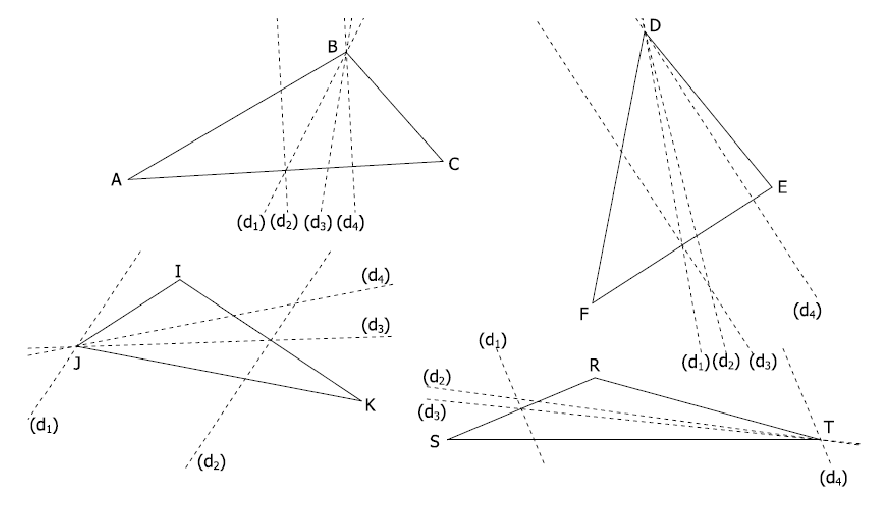
\includegraphics[scale=1]{mediatrices.eps} 

\q Quel est le signe du produit de 150 facteurs tous égaux à (– 1) ? \textbf{Justifier}. \\

\q Quelle est le signe d'un produit de 65 facteurs dont 25 sont positifs? \textbf{Justifier}. \\


\vspace*{0.6cm}



\exo{2}\\

Calculer en regroupant les facteurs de façon astucieuse (faire apparaître les regroupements sur votre feuille).\\

$R = (-2) \times 25 \times (-5) \times(-4) \times (-0,01)$\\

\vspace*{0.6cm}



\exo{7}\\

Calculer les expressions suivantes en écrivant \textbf{toutes} les étapes intermédiaires  :\\

\bmul{3}

$F= (-2,5) \times (-4)$\\

$H=-5 + 4 \times (-3)$\\

\columnbreak

$U= 11 -28 \div(-7)$\\

$E=\dfrac{-3 -(-4)\times 12}{-3-2}$\\

\columnbreak

$R= 72 \div 8 \div 3 \times 4$\\

$V= 6-[(-4) \times (-3) + 5 \times (-2)]\times (-4)$\\


\emul


\exo{1}
Un bathyscaphe se déplace dans le golfe du Mexique, profond de 3 787 m. Il s'enfonce d'abord de -900 mètres puis descend encore du triple de cette profondeur.\\

Quelle profondeur a-t-il alors atteint ? \textbf{Justifier} la réponse par un calcul. \\



\newpage

\exo{3,5}\\

\initq 
\q Construire un triangle ABC tel que : AB = 4cm ; AC = 7 cm et BC = 8 cm. 
Tracer la hauteur issue du point A. Elle coupe le segment [BC] au point H. Placer le point I, milieu du segment [AB].\\


\q Calculer la longueur HI. \textbf{Justifier} la réponse en utilisant les propriétés du cours.\\

\vspace*{0.6cm}


\exo{2,5}\\


\bmul{2}

$(C)$ est le cercle de diamètre [AB] et D est un point du cercle $(C)$.\\

\initq 
\q Démontrer que le triangle ABD est un triangle rectangle en D.\\

\q En déduire la mesure de l'angle $\widehat{BAD}$. Justifier votre réponse.
\columnbreak

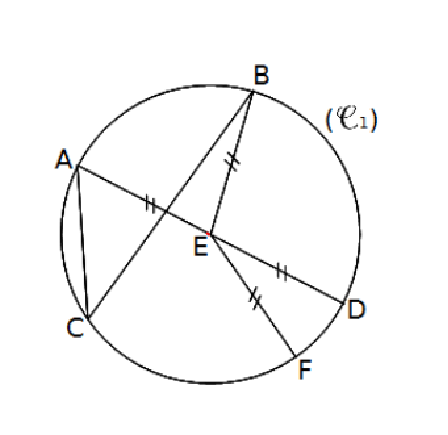
\includegraphics[scale=1]{cercle.eps} 

\emul

\vspace*{0.6cm}


\exo{1}(\textbf{Sur le sujet})\\

\bmul{2}

Dans un jardin public qui a la forme d’un triangle RST,
les élus de la ville veulent installer une statue qui soit à
égale distance de chaque sommet.\\
Sur le plan de ce jardin, construire avec précision
l'emplacement M de la statue.

\columnbreak


\includegraphics[scale=1]{triangle.eps} 

\emul

\exo{} Bonus \\

\initq 

\q Calculer la somme de 48 facteurs tous égaux à (-2). Justifier votre réponse par un calcul.\\

\q L'égalité $x^{2} -5 = 1-x$ est-elle vraie pour : $x=-3$, $x=-1$ ou $x=2$? Justifier votre réponse par un calcul.




\end{document}
